\chapter[Resultados]{Resultados}

\section{Análise teórica vs. Otimização do painel reforçado}
Esta seção está dividida em três subseções:
\begin{itemize}
\item Resultados da análise teórica do painel reforçado;
\item Resultados da otimização do painel reforçado fabricado em material metálico;
\item Comparação dos dois itens ateriores .
\end{itemize}

\subsection{Análise teórica do painel reforçado}
A análise teórica do painel reforçado seguiu a metodologia do \emph{Fator de Eficiência de Farrar} proposta por \cite{niu1997airframe}. O painel reforçado foi submetido a uma carga de compressão de intensidade 10000daN (269777lbs), obtendo-se portando uma carga de compressão linear (N) como segue:\\~\\

\centerline{N = 1000 N/mm = 5710.2 lbs/in}\

Utilizou-se os seguintes valores na análise teórica:
F=0.65; $R_t$=1.50; $R_b$=0.33;
Da \autoref{fig_plotFarrar}, encontrou-se o valor de "f" correspondente a carga por largura (5710.4 lbs/in), utilizando F=0.65 para o Al 2024-T3 extrudado.\\~\\

\centerline{f = 40000 psi}\

Encontrou-se o módulo tangente $E_t$, aproximado, correspondente ao valor de "f", da curva de módulo tangente do material, conforme \autoref{fig_tangentmodulus}.\\~\\

\centerline{$E_t$ = 5.4x$10^6$ psi}
\

Conforme \autoref{fig_plotstiffener2}, determinou-se o valor de $J_4$:

\centerline{$J_4$ = 1.2}\

E determinou-se o valor $t$ e $t_w$, como segue:\\~\\

\centerline{$t = J_4({\dfrac{NL}{E_t}})^{0.5} = 0.153 in = 3.884 mm$}\

\centerline{$t_w = {R_t}t= 1.2t = 0.183in = 4.661 mm$}\


\subsection{Otimização do painel reforçado em material metálico}
Desenvolveu-se um modelo de otimização do reforçador em material metálico, no qual, o material possuia as mesmas propriedades de módulo de elasticidade tangente ($E_t$) do modelo teórico, visto que a solução 105 do \emph{Nastran} é linear, ou seja, não leva em conta a plasticidade do material. Para este modelo, encontrou-se o seguinte resultado:\

\centerline{$t = 2.544 mm$}\

\centerline{$t_w = 5.724 mm$}\

\begin{figure}[ht]
 \caption{\label{fig_ModelMetallic}Resultado do reforçador em material metálico.}
 \centering
 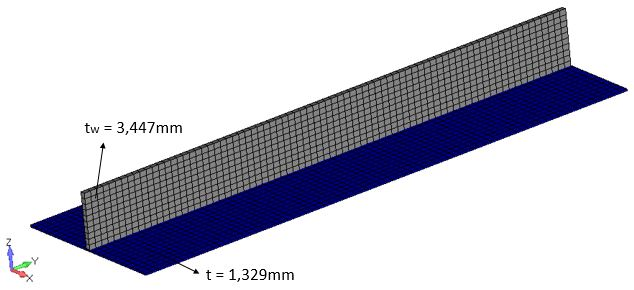
\includegraphics[scale=1.0]{figura/Model_Metallic1}
\end{figure}
\

\subsection{Comparação dos resultados}
A \autoref{tbl:result1_metalico} seguinte compara os resultados das espessuras do revestimento e do reforçador obtidas na análise do modelo teórico e do modelo otimizado.
\begin{table}[h]
\centering
\begin{tabular}{ccc}
\toprule
Modelo & Revestimento (mm) & Reforçador (mm) \\\midrule
Teórico & 3.884 & 4.661\\
Otimizado & 2.544 & 5.724\\
\bottomrule
\end{tabular}
\caption{Resultados de espessuras.}
\label{tbl:result1_metalico}
\end{table}

Tendo-se como base a geometria do reforçador e a densidade mássica do material considerado, calculou-se as massas das estruturas. E os resultados são conforme mostrado na \autoref{tbl:result2_metalico}.

\begin{table}[h]
\centering
\begin{tabular}{cc}
\toprule
Modelo & Massa (kg) \\ \midrule
Teórico & 0.717\\
Otimizado & 0.587\\
\bottomrule
\end{tabular}
\caption{Resultados de massa da estrutura.}
\label{tbl:result2_metalico}
\end{table}

Observa-se que foram encontradas espessuras, e consequentemente, massas das estruturas diferentes, entre os modelos teóricos e o modelo da otimização.
Em relação as massas foi encontrada uma diferença de 18.12\%. Essa diferença se deve ao fato de o modelo teórico ter considerado um reforçador ótimo com o fator de eficiência de Farrar de 0.65, e caso esse fator pudesse ser melhorado, o modelo teórico ficaria mais aproximado do modelo otimizado.

\section{Análise teórica vs. Otimização do painel reforçado}
Esta seção está dividida em três subseções:
\begin{itemize}
\item Resultados da otimização do painel reforçado fabricado em material metálico;
\item Resultados da otimização do painel reforçado fabricado em material composto;
\item Comparação dos dois itens ateriores .
\end{itemize}

\subsection{Otimização do painel reforçado em material metálico}
Desenvolveu-se um modelo de otimização do reforçador em material metálico, no qual, o material possuia as propriedades conforme mostrado na \autoref{tbl:prop_metalico}. A carga de compressão aplicada neste modelo se deu da mesma forma mostrada na \autoref{fig_StiffMetalLoad}, no entanto com o módulo de 10000daN. Para este modelo, do reforçador constituído de material metálico, encontrou-se o seguinte resultado:\

\centerline{$t = 3.092 mm$}\

\centerline{$t_w = 2.165 mm$}\

\centerline{$t_{wBase} = 4.174 mm$}\

\begin{figure}[ht]
 \caption{\label{fig_Result1Metallic}Resultado do reforçador em material metálico.}
 \centering
 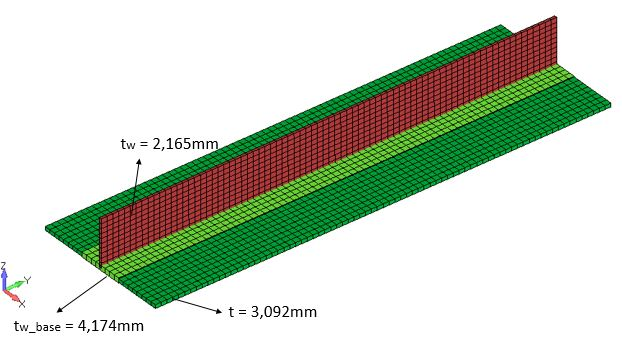
\includegraphics[scale=0.8]{figura/Results_Metallic}
\end{figure}
\

%Em relação ao resultado da análise de flambagem, a \autoref{fig_Result2Metallic} mostra a resposta da estrutura com o primeiro autovalor encontrado para este reforçador em material metálico.

%\begin{figure}[ht]
% \caption{\label{fig_Result2Metallic}Análise de flambagem do reforçador em material metálico ($\lambda_1 = 1.021$).}
% \centering
% 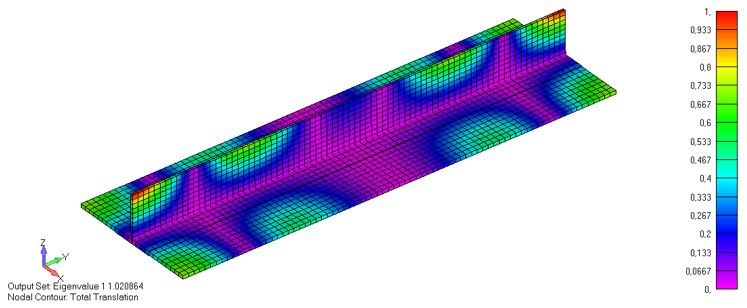
\includegraphics[scale=0.85]{figura/Results2_Metallic}
%\end{figure}
%\

\subsection{Otimização do painel reforçado em material composto}

Desenvolveu-se um modelo de otimização do reforçador em material composto, no qual, os propriedades do material variavam com base na otimização dos parâmetros de laminação. A carga de compressão aplicada no modelo do reforçador de material composto foi a mesma aplicada no modelo metálico, com o módulo de 10000daN. Para este modelo, encontrou-se o seguinte resultado para as espessuras:\

\centerline{$t = 2.928 mm$}\

\centerline{$t_w = 2.611 mm$}\

\centerline{$t_{wBase} = 4.234 mm$}\

E encontrou-se o seguinte resultado para os parâmetros de laminação:\

\begin{table}[h]
\centering
\begin{tabular}{ccccc}
\toprule
Estrutura & $\xi^A_{1}$ & $\xi^A_{2}$ & $\xi^D_{1}$ & $\xi^D_{2}$ \\ \midrule
Reforçador & 0.3182 & 0.0348 & 0.0537 & -0.0625\\
Revestimento & 0.2560 & 0.0529 & -0.0851 & -0.0913\\
Base reforçador & 0.2853 & 0.0443 & 0.0215 & -0.199\\
\bottomrule
\end{tabular}
\caption{Resultados dos parâmetros de laminação.}
\label{tbl:result_qsis}
\end{table}


\begin{figure}[ht]
 \caption{\label{fig_Result1Composite}Resultado do reforçador em material composto.}
 \centering
 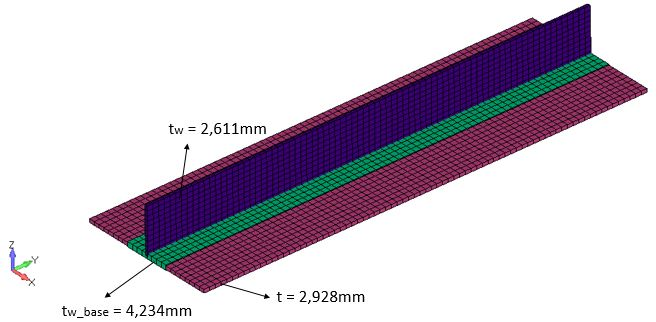
\includegraphics[scale=0.8]{figura/Results_Composite}
\end{figure}
\

Em relação ao resultado da análise de flambagem, a \autoref{fig_Result2Composite} mostra a resposta da estrutura com o primeiro autovalor encontrado para este reforçador em material composto.

\begin{figure}[ht]
 \caption{\label{fig_Result2Composite}Análise de flambagem do reforçador em material composto ($\lambda_1 = 1.021$).}
 \centering
 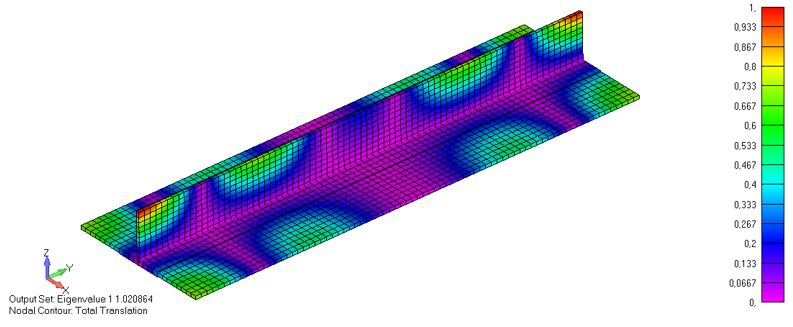
\includegraphics[scale=0.85]{figura/Results2_Composite}
\end{figure}
\

\subsection{Comparação dos resultados}

A \autoref{tbl:result1_composto} compara os resultados das espessuras do revestimento, do reforçador e da base do reforçador obtidas na otimização do modelo em material metálico e do modelo em material composto.
\begin{table}[h]
\centering
\begin{tabular}{cccc}
\toprule
Modelo & Revestimento (mm) & Reforçador (mm) & Base do reforçador (mm) \\\midrule
Metálico & 3.092 & 2.165 & 4.174 \\
Composto & 2.928 & 2.611 & 4.234\\
\bottomrule
\end{tabular}
\caption{Resultados de espessuras.}
\label{tbl:result1_composto}
\end{table}

Tendo-se como base a geometria do reforçador e a densidade mássica dos materiais, sendo $\rho_{metal} =$ $2.8$x$10^{-3} g/mm^3$ e $\rho_{composto} =$ $1.56$x$10^{-3} g/mm^3$ calculou-se as massas das estruturas. E os resultados são conforme mostrado na \autoref{tbl:result2_composto}.

\begin{table}[h]
\centering
\begin{tabular}{cc}
\toprule
Modelo & Massa (kg) \\ \midrule
Teórico & 0.551\\
Otimizado & 0.309\\
\bottomrule
\end{tabular}
\caption{Resultados de massa da estrutura.}
\label{tbl:result2_composto}
\end{table}

Observa-se que foram encontradas espessuras e massas das estruturas diferentes, entre os modelos de otimização do reforçador em material metálico e o reforçador em material composto.
Em relação a massa da estrutura, que era a função objetivo da otimização, a otimização do reforçador em material composto gerou um resultado de uma estrutura com a massa 43\% menor do que o reforçador em material composto. Isto mostra, portanto, que para a situação e modelo considerados, o reforçador em material composto é mais eficiente do que o reforçador em material metálico, visto que ambos suportam a mesma carga de flambagem, no entanto, o reforçador em material composto possui uma massa estrutural menor.
